\section{Results}
\label{sec:results}

\subsection{Social IQA Measures Local Fidelity}

\begin{table}[t]
\centering
\caption{\socialiqa local-fidelity results. Higher is better for accuracy and macro-F1. Best values are in \textbf{bold}.}
\label{tab:social_iqa}
\resizebox{\linewidth}{!}{%
\begin{tabular}{@{}lccccc@{}}
\toprule
Condition & $N$ & Accuracy & 95\% CI & Macro-F1 & Entropy (bits) \\
\midrule
Demographic & 90 & 0.700 & [0.600, 0.778] & 0.701 & 1.583 \\
Persona & 90 & \textbf{0.789} & [0.700, 0.867] & \textbf{0.789} & \textbf{1.583} \\
Unconditioned & 90 & 0.744 & [0.644, 0.822] & 0.744 & 1.581 \\
\bottomrule
\end{tabular}%
}
\end{table}


\Figref{fig:social_iqa_dist} reports the aggregate answer counts, and \tabref{tab:social_iqa} reports the summary metrics. Persona conditioning achieves the best local fidelity, reaching 0.789 accuracy and 0.789 macro-F1. This is a 4.4-point improvement over the unconditioned baseline and an 8.9-point improvement over demographic conditioning. The paired comparison between persona and demographic prompting yields an exact McNemar-style proxy of $p=0.0215$, while persona versus unconditioned is smaller and not significant at the 0.05 level ($p=0.2891$).

The main surprise is that conditioning changes accuracy more than it changes the aggregate answer distribution. Answer entropy is nearly constant across all three conditions at about 1.58 bits, and pairwise Jensen-Shannon divergences are tiny, ranging from 0.0004 to 0.0022. In other words, persona prompts improve which items the model gets right without substantially changing the overall mix of A/B/C selections. This supports local fidelity and some latent-factor responsiveness, but it does not yet show broad distributional change.

\begin{figure}[t]
\centering
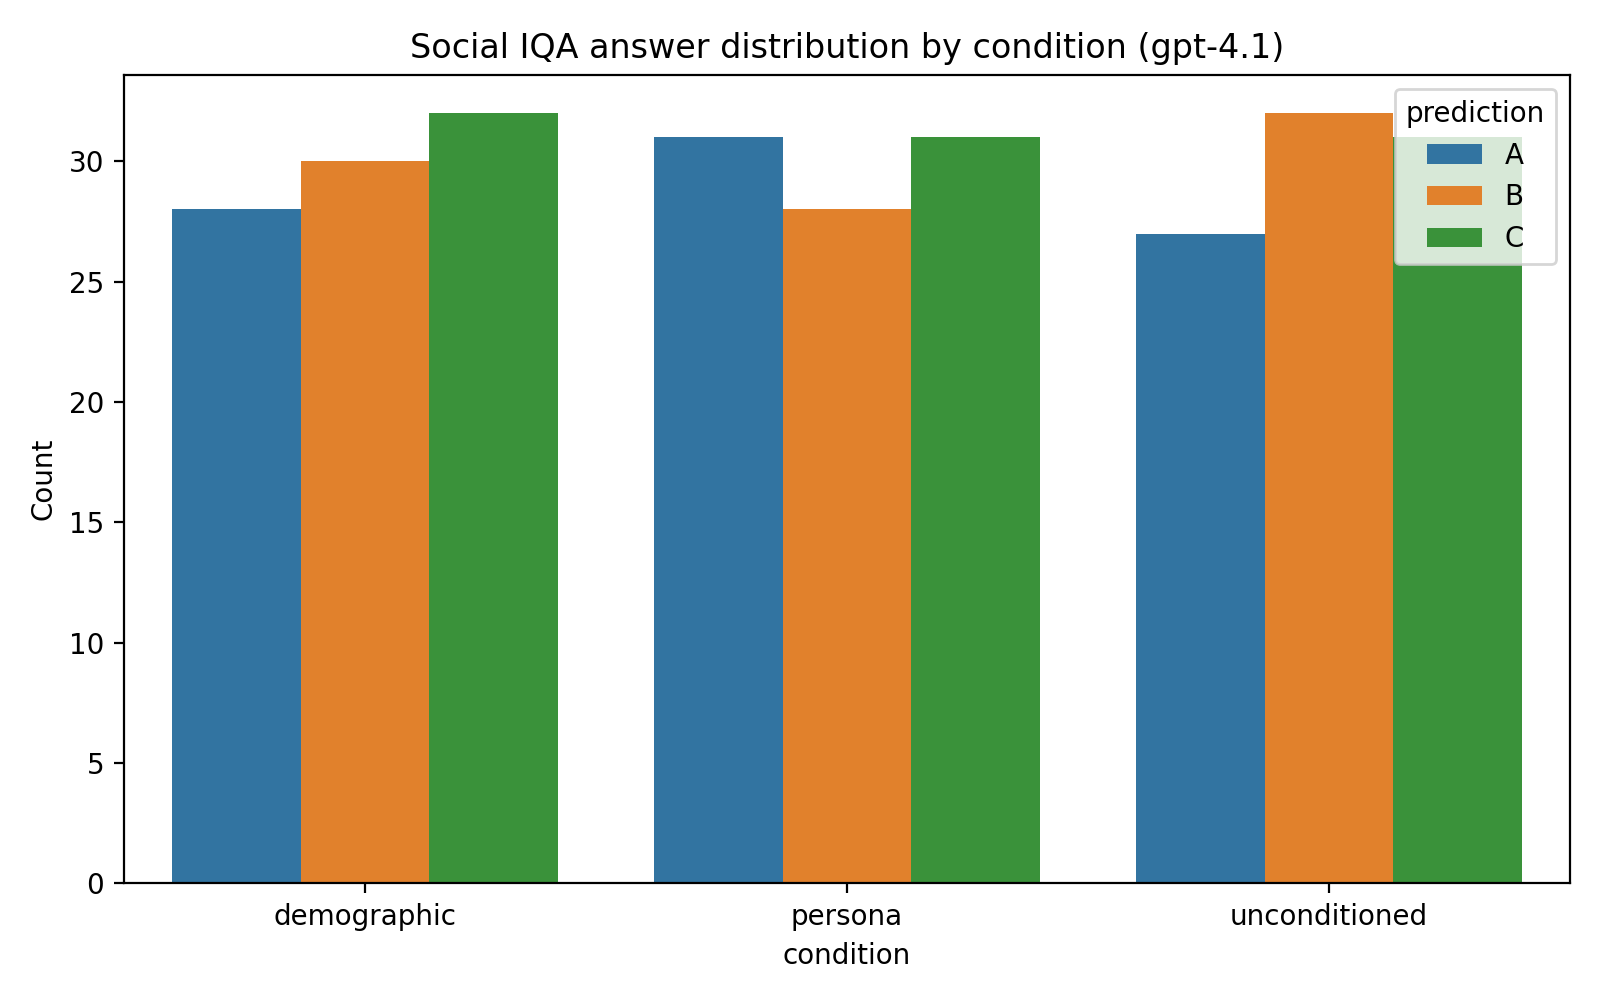
\includegraphics[width=0.92\linewidth]{figures/social_iqa_distribution_gpt-4.1.png}
\caption{Aggregate \socialiqa answer counts by prompt condition. Persona conditioning improves item-level accuracy, but the aggregate choice distribution remains almost unchanged, consistent with the very small pairwise Jensen-Shannon divergences.}
\label{fig:social_iqa_dist}
\end{figure}

\subsection{Ultimatum Policies Broaden Slightly but Remain Compressed}

\begin{table}[t]
\centering
\caption{Ultimatum-game simulation results. Higher threshold standard deviation and more distinct profiles indicate broader behavioral support, while monotonicity violations should remain low. Best values are in \textbf{bold} within each column.}
\label{tab:ultimatum}
\resizebox{\linewidth}{!}{%
\begin{tabular}{@{}lcccccc@{}}
\toprule
Condition & Participants & Mean threshold & 95\% CI & Threshold SD & Policy entropy & Distinct profiles \\
\midrule
Demographic & 15 & 2.40 & [2.13, 2.67] & 0.51 & 0.608 & 2 \\
Persona & 15 & 2.53 & [1.93, 3.00] & \textbf{1.13} & 0.590 & \textbf{5} \\
Unconditioned & 15 & \textbf{2.67} & [2.40, 2.87] & 0.49 & \textbf{0.677} & 2 \\
\bottomrule
\end{tabular}%
}
\end{table}


\Figref{fig:ultimatum_curves} shows the acceptance curves, and \tabref{tab:ultimatum} reports participant-level summaries. All three conditions produce monotone or nearly monotone policies, which means the simulator behaves consistently as offers improve. However, the thresholds are unrealistically low in every condition. Demographic prompting yields a mean threshold of 2.40, persona prompting 2.53, and unconditioned prompting 2.67. Every condition accepts offers of 3 or more almost universally.

Persona conditioning does widen behavioral support. It increases the threshold standard deviation from about 0.5 to 1.13 and raises the number of distinct policy profiles from 2 to 5. The persona condition is also the only one that produces an always-accept policy and a stricter \texttt{RRRAAAAAA} profile. Yet this additional variety still sits within a narrow family of cooperative policies. Even the strictest observed profile begins accepting at offer 3, and one persona accepts every offer from 1 through 9. The model therefore broadens the manifold without recovering human-like tails.

The pairwise threshold intervals reinforce this conclusion. Unconditioned prompting produces a modestly higher mean threshold than demographic prompting, with a difference of 0.267 and a 95\% interval of [0.178, 0.351]. By contrast, persona versus demographic and persona versus unconditioned both include zero. Conditioning changes the support more than it changes the central tendency.

\begin{figure}[t]
\centering
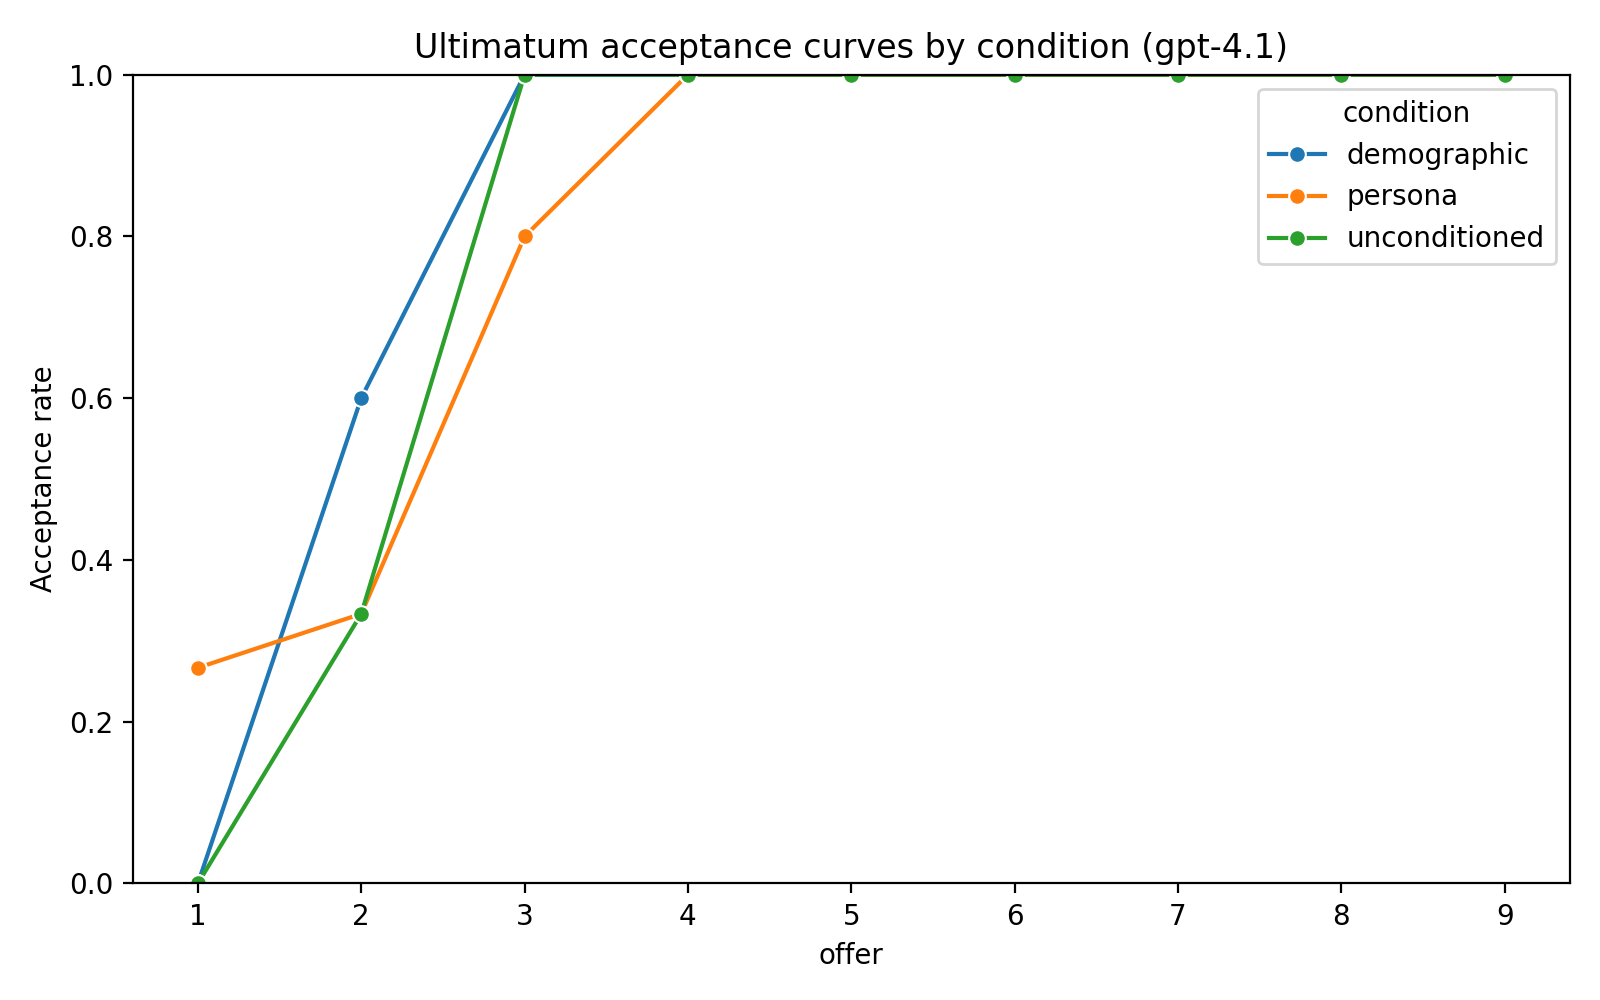
\includegraphics[width=0.92\linewidth]{figures/ultimatum_curves_gpt-4.1.png}
\caption{Acceptance curves in the ultimatum game. Persona conditioning produces the widest range of participant policies, but all three conditions accept unfair offers far earlier than expected from human populations, with near-universal acceptance by offer 3 or 4.}
\label{fig:ultimatum_curves}
\end{figure}

\subsection{Token Usage}

The study is lightweight in monetary terms. \socialiqa used 52{,}524 tokens, and the ultimatum benchmark used 73{,}333 tokens, for a combined total of 125{,}857 tokens. Using the official May 5, 2026 pricing for \gptfourone, this corresponds to about \$0.151 for \socialiqa, \$0.215 for ultimatum, and \$0.366 overall \cite{openai2026gpt41,openai2026pricing}. The low cost makes this style of evaluation easy to repeat across models, which is useful because simulation validity is likely to change over time.
